\documentclass{article}
\usepackage[utf8]{inputenc}
\usepackage{graphicx}
\title{Actividad 3 Fortran}
\author{Glenda Carranco}
\date{September 2019}

\begin{document}

\maketitle

\section{Introduction}
En esta nueva actividad aprendimos como integrar un nuevo "codigo" para hacer repeticiones llamado do-loop que nos ayudara a calcular de manera mas eficiente diferentes datos.

\section{Parte 1}
Primero usamos el mismo codigo de la actividad 2:
\begin{verbatim}
    program projectile
  implicit none

  ! definimos constantes
  real, parameter :: g = 9.8
  real, parameter :: pi = 3.1415927

  ! definimos las variables
  real :: a, t, u, x, y
  real :: theta, v, vx, vy

  ! Leer valores para el ángulo a, el tiempo t, y la velocidad inicial u desde la terminal
  write(*,*) 'Dame el ángulo, el tiempo y la rapidez inicial'
  read(*,*) a, t, u

  ! convirtiendo ángulo a radianes
  a = a * pi / 180.0
  
  ! las ecuaciones de la posición en x y y
  x = u * cos(a) * t
  y = u * sin(a) * t - 0.5 * g * t * t

  ! La velocidad al tiempo t
  vx = u * cos(a)
  vy = u * sin(a) - g * t
  v = sqrt(vx * vx + vy * vy)
  theta = atan(vy / vx) * 180.0 / pi
 
 ! escribiendo el resultado en la pantalla
  write(*,*) 'x: ',x,'  y: ',y
  write(*,*) 'v: ',v,'  theta: ',theta

end program projectile
 
\end{verbatim}

Lo modificamos y agregamos un "do loop" que calcula la posicion del proyectil cada 0.1 segundos:
\begin{verbatim}
     ! Numero de puntos Grafica
  PRINT*,"Dame el numero de pasos que quieres en la parabola"
  Read*,npasos
  OPEN(1,FILE="SALIDAS.DAT" ,ACCESS="APPEND")
  Do j = 1,6
  ang=float(m)*dtang
  Do i=0 ,npasos
   t=float(i)*dt
  !IF(y<0.0)EXIT
  
\end{verbatim}

Con un programa llamado "Gnuplot" logramos primeros resultados:



Déspues nos pidieron que modificaramos el doo loop para que calculara la posición en diferentes ángulos:

\begin{verbatim}
    
  ! Numero de puntos Grafica

  OPEN(unit=11 ,FILE="SALIDAS.DAT" ,status="unknown")
  Do j = 1,6
  a=float(j)*dtang
  Do i=0 ,200
   t=(i)*dt
  
  
  !las ecuaciones de la posición en x y y
  x = u * cos(a) * t
  y = u * sin(a) * t - 0.5 * g * t * t
 
	IF(y<0.0)EXIT

  WRITE(11,*)x,y
  End do
  WRITE(11,*) " "
  End do
  close (11)
 
\end{verbatim}

y usamos Gnuplot para volver a calcular la grafica


    \centering
    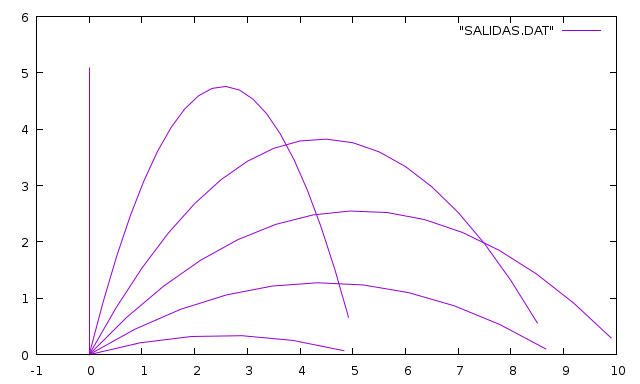
\includegraphics[scale=0.5]{grafica1.png}
    \caption{graphic 2}
    \label{fig:my_label}
    
    Como podemos verla grafica son varias parabolas que muestran como fue el movimiento en varios puntos.


















\end{document}
